\chapter{Vereinheitlichung zweier Messungen des \texorpdfstring {$t\bar{t}\gamma$}{math} Produktionswirkungsquerschnitts mit dem EFTfitter}%
In diesem Kapitel erfolgt die Kombination der Messungen von ATLAS und CMS für den $t\bar{t}\gamma$ Produktionswirkungsquerschnitt bei einer Schwerpunktsenergie von $\sqrt{s} = \SI{8}{\tera\electronvolt}$. Da die Messungen in unterschiedlichen Phasenräumen erfolgt sind, wird vor der eigentlichen Kombination mit dem EFTfitter eine Phasenraumstudie durchgeführt, um die Phasenräume zu vereinheitlichen.

\section{\texorpdfstring {$t\bar{t}\gamma$}{math} Messungen von ATLAS und CMS}%
\label{kap:messung}
Die Messungen des Produktionswirkungsquerschnitts von ATLAS\cite{Aaboud:2017era} und CMS\cite{Sirunyan:2017iyh} sind beide bei einer Proton-Proton-Kollision bei einer Schwerpunktsernegie von $\sqrt{s}=\SI{8}{\tera\electronvolt}$ durchgeführt worden. Die Bestimmung des Wirkungsquerschnitts erfolgt über den semileptonischen Endzustand. Somit zerfällt eins der entstehenden $W$-Bosonen in ein Elektron oder Myon mit dem entsprechenden Neutrino und das andere $W$-Boson hadronisch. Ein möglicher Feynman-Graph für diesen Prozess ist in~\ref{fig:tta} dargestellt.\\
Obwohl ATLAS und CMS den gleichen Prozess betrachtet haben, unterscheiden sich die Messungen grundlegend durch den zu Grunde liegenden gemessenen Phasenraum. Die Wahl den gemessenen Phasenraum zu betrachten, hat den Vorteil, dass die Modellunabhängigkeit maximiert wird und die Extrapolation in den experimentell nicht messbaren Phasenraum minimiert wird. Die von ATLAS und CMS verwendeten Schnitte für ihren gemessenen Phasenraum sind in Tabelle \ref{tab:cut}
aufgeführt.\\
%
 \begin{table}[H]
     \centering
    \begin{tabular}{c|l|l}
      Objekte & ATLAS & CMS \\
      \hline
      \textbf{Photon} & $p_T > \SI{15}{\giga\electronvolt}\quad |\eta| < 2,37$ & $p_T > \SI{25}{\giga\electronvolt}\quad |\eta| < 1,44$\\
      Leptonen & $p_T > \SI{25}{\giga\electronvolt}\quad |\eta| < 2,5$ & $\text{e}:\: p_T > \SI{35}{\giga\electronvolt}\quad |\eta| < 2,5$ \\
      {} & {} & $\symup{\mu}:\: p_T > \SI{26}{\giga\electronvolt}\quad |\eta| < 2,5$\\
      Jets & $p_T > \SI{25}{\giga\electronvolt}\quad |\eta| < 2,5$ & $p_T > \SI{30}{\giga\electronvolt}\quad |\eta| < 2,4$\\
      b-Jets & $p_T > \SI{5}{\giga\electronvolt}$ &  \\
      Neutrino &  & $p_T^{miss} > \SI{20}{\giga\electronvolt}$
    \end{tabular}
    \caption{Verwendete Schnitte auf den gemessenen Phasenraum.}
    \label{tab:cut}
 \end{table}
Dabei fällt auf, dass die Schnitte für das Photon sich deutlich unterscheiden. So setzt ATLAS einen Transversalimpuls von $p_{T} > \SI{15}{\giga\electronvolt}$ voraus, wohingegen CMS mindestens $p_{T} > \SI{25}{\giga\electronvolt}$ einfordert. Außerdem wählt ATLAS eine Pseudorapidität von $|\eta| < 2,37$, während CMS $|\eta| < 1,44$ annimmt. Zudem setzt CMS einen durch das Neutrino fehlenden Transversalimpuls von $p_{T}^{miss} > \SI{20}{\giga\electronvolt}$ voraus.
ATLAS setzt zudem zwischen dem Photon und dem Lepton mindestens ein Abstand von $\symup{\Delta} R(\gamma, \text{l}) = 0,7$, zwischen dem Photon und dem Jet $\symup{\Delta} R(\gamma, \text{Jet}) = 0,5$ und zwischen dem $b$-Quark und dem Jet $\symup{\Delta} R(\text{b}, \text{Jet}) = 0,3$ vorraus.
Das CMS Papier umfasst keine weiteren Angaben zur Isolation der Objekte.\\
Die von ATLAS und CMS gemessenen Produktionswirkungsquerschnitte für $t\bar{t}\gamma$ ergeben sich zu:
\begin{align*}
  \sigma^{fid, \text{ATLAS}}_{t\bar{t}\gamma} &= 139 \pm 18~\text{(stat.$+$syst.)}~ \si{\femto\barn}\\
  \sigma^{fid, \text{CMS}}_{t\bar{t}\gamma, e} &= 138 \pm 45~\text{(stat.$+$syst.)}~ \si{\femto\barn}\\
  \sigma^{fid, \text{CMS}}_{t\bar{t}\gamma, \mu} &= 115 \pm 32~\text{(stat.$+$syst.)}~ \si{\femto\barn}.
\end{align*}
CMS unterscheidet dabei zwischen zwei Wirkungsquerschnitten, bei denen das Lepton im Endzustand einmal ein Elektron und einmel ein Myon ist.

\section{Kombinationen mit dem EFTfitter}
Der EFTfitter\cite{Castro:2016jjv} ist ein Programm, das es ermöglicht Studien zur BSM-Physik auf Grundlage von effektiven Feldtheorien durchzuführen. Er erlaubt Benutzern physikalische Modelle selbst zu implementieren und im
Zusammenhang der Wahrscheinlichkeitsrechnung nach Bayes zu testen. Zudem ist eine Kombination verschiedener Messungen möglich, ohne diese selbst durchgeführt zu haben.
Bei solchen Kombinationen ist die Breite der Wahrscheinlichkeitsverteilung und damit ihre Aussagekraft von der Anzahl der Messungen abhängig.
Die Bayessche Inferenz ermöglicht eine Anpassung des Modells an die Daten, sodass eine Wahrscheinlichkeitsverteilung für den gesuchten Parameter des Modells erhalten wird.\\
Die Grundlage für diese Berechnungen liefert der Satz von Bayes:
\begin{align}
  p(\lambda|x) = \frac{L(x|\lambda) \cdot \pi(\lambda)}{p(x)}.
\end{align}
Der gesuchte Parameter des Modells ist $\lambda$ und die verwendete Datenmenge wird in diesem Fall durch $x$ beschrieben. Die A-Prioriverteilung $\pi(\lambda)$ enthält Informationen über die zu untersuchende Variable $\lambda$. Dies können zum Beispiel physikalische Konstanten sein, die zum Implementieren des Modells benötigt werden.
Die Normierung $p(x)$ wird mit:
\begin{align}
  p(x) = \int d\lambda L(x|\lambda) \cdot \pi(\lambda)
\end{align}
berechnet. Die Likelihood $L(\vec{x}|\lambda)$ beschreibt die Wahrscheinlichkeitsverteilung der Daten $\vec{x}$. Die gesuchte Posteriorverteilung wird durch $p(\lambda|\vec{x})$ beschrieben. Diese beinhaltet neue Erkenntnisse über den Parameter $\lambda$, die aus den Daten gewonnen werden. Somit kann die anfängliche Erkenntnis über den Parameter $\lambda$ verbessert werden.\\
Werden für eine Kombination $n$ Messungen $x_i$ mit $(i= 1,...,n)$ und $N$ Observablen $y_i$ mit $(i= 1,...,N)$ betrachtet, kann die Likelihood als gaußförmig angenommen werden und wird mit:
\begin{align}
  -2 \ln{L(\mathbf{x}|\lambda)} = \sum^{n}_{i=1} \sum^{n}_{j=1} \left[\mathbf{x} - U\mathbf{y}\right]_{i} \mathcal{M}_{ij}^{-1} \left[\mathbf{x} - U\mathbf{y}\right]_{j}
  \label{eqn:like}
\end{align}
beschrieben. $U_{ij}$ ist das Matrixelement einer $n \times N$-Matrix $U$, welches eins ist, wenn $x_i$ die Messung zur Observable $y_i$ ist und ansonsten null. Da die Unsicherheiten der Messung $x_i$ korreliert sein können, beschreibt
\begin{align}
  \mathcal{M}_{ij} = \text{cov}[x_i, x_j] = \sum_{k=1}^{M} \text{cov}^{(k)}[x_i, x_j]
\end{align}
die Elemente der symmetrischen und positiv semidefiniten Kovarianzmatrix, bei der $M$ die Anzahl der verscheidenen Quellen an Unsicherheiten ist. Das mit dem EFTfitter berechnete Ergebnis wird ebenfalls bei der Verwendung der BLUE-Methode (\textit{best linear unbiased estimator})\cite{LYONS1988110} erhalten. Da diese einen Spezialfall des EFTfitter bildet und einer Minimierung der Likelihood \eqref{eqn:like} entspricht.

\section{Phasenraumstudie mit MadGraph5}
\label{phasencms}
Um eine Kombination der beiden Messungen des $t\bar{t}\gamma$ Wirkungsquerschnitts von CMS und ATLAS ermöglichen zu können, muss zuvor eine Phasenraumstudie durchgeführt werden. Da beide Messungen in unterschiedlichen Phasenräumen durchgeführt wurden, müssen sie zunächst vereinheitlicht werden.
Der Vergrößerung eines Phasenraums liegt ein linearer Zusammenhang zu Grunde, sodass als erste Approximation ein Faktor zwischen den beiden Phasenräumen bestimmt werden kann. Dazu können mit Hilfe des Monte Carlo Generators MadGraph5\cite{Alwall:2014hca} (MG) zunächst die beiden Produktionswirkungsquerschnitte für $t\bar{t}\gamma$ berechnet werden.
Anschließend werden diese beiden Werte durcheinader geteilt und der sich ergebene Faktor wird auf die CMS-Messung angewandt. Dadurch wird diese Messung in den Phasenraum der ATLAS Messung erweitert.\\
Zunächst einmal wird der semileptonische Zerfall des $t\bar{t}$-Quarkpaars unter Abstrahlung des Photons mit den expliziten Endzuständen in MG simuliert. Dazu wird das SM als Modell und das $\text{CTEQ}6\text{L}1$ PDF Set\cite{Paakkinen:2018zbs} zum Implementieren des Prozesses genutzt. Bei der Berechnung der semileptonischen Endzustände kann jedoch nur die führende Ordnung (\textit{leading-order}, LO) betrachtet werden. Für die Berechnung der Produktionswirkungsquerschnitte werden die in Kapitel \ref{kap:messung} angegebenen Schnitte genutzt. Da von der CMS-Kollaboration in dem Papier keine weiteren Aussagen über die Isolation der einzelnen Objekte gemacht werden, werden für diese Arbeit die gleichen Abstände wie bei ATLAS verwendet. Unter diesen Vorraussetzungen ergeben sich die Wirkungsquerschnitte aus der MG Simulation zu:
\begin{align}
  \sigma^{fid, \text{ATLAS}}_{\text{LO}} &= 146,5 \pm 0,095~ \si{\femto\barn}\\
  \sigma^{fid, \text{CMS}}_{\text{LO}} &= 49,29 \pm 0,034~ \si{\femto\barn}.
\end{align}
Auffällig ist dabei, dass der Wert von ATLAS $2,97$ mal so groß ist, wie der CMS Produktionswirkungsquerschnitt. Dies ist unerwartet, da beide Ergebnisse der Messungen sehr ähnlich sind und in den Papieren als vertäglich mit dem SM angesehen werden.
Beim Vegleich der Photon-Schnitte fällt jedoch auf, dass durch den höheren $p_T$-Schnitt von CMS bereits ungefähr $90000$ der anfänglichen $220000$ Ereignisse verloren gehen. Durch den Schnitt auf die Pseudorapidität entfallen ebenfalls nochmal etwa $45000$ Ereignisse. Dies entspricht etwa $\SI{60}{\percent}$ der anfänglichen Ereignisse, sodass der Faktor $3$ durchaus plausibel erscheint. Eine Veranschaulichung dieser Änderungen befindet sich in Abbildungildung \ref{fig:schnitte}.\\
\begin{figure}
    \begin{subfigure}[c]{0.5\textwidth}
      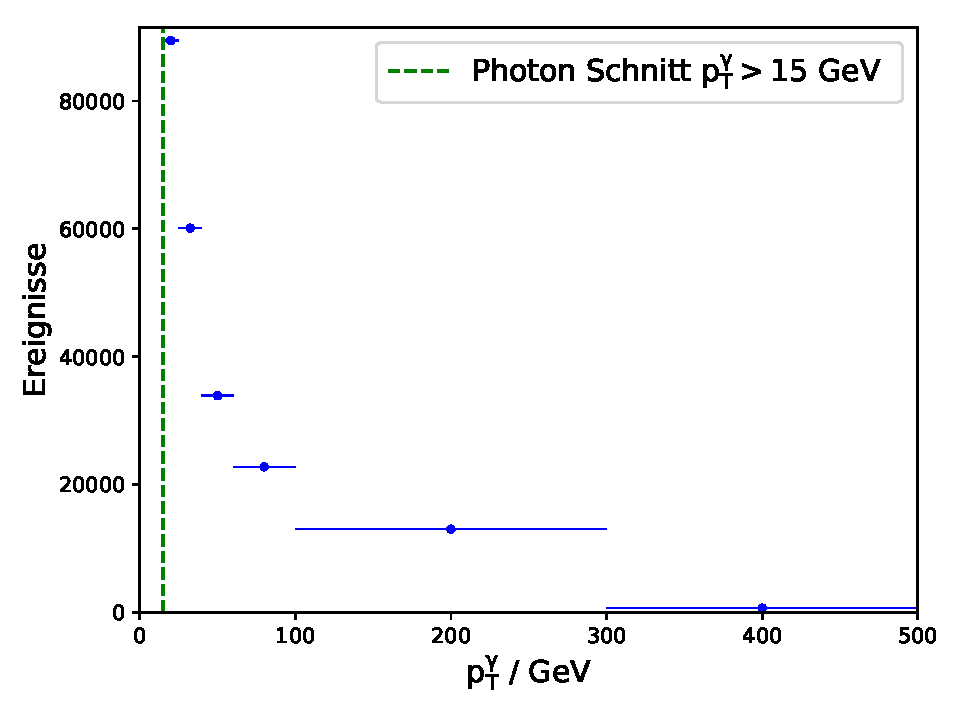
\includegraphics[width=\textwidth]{Plots/photon_pt_Atlas.pdf}
      \subcaption{ATLAS}
    \end{subfigure}
    \begin{subfigure}[c]{0.5\textwidth}
      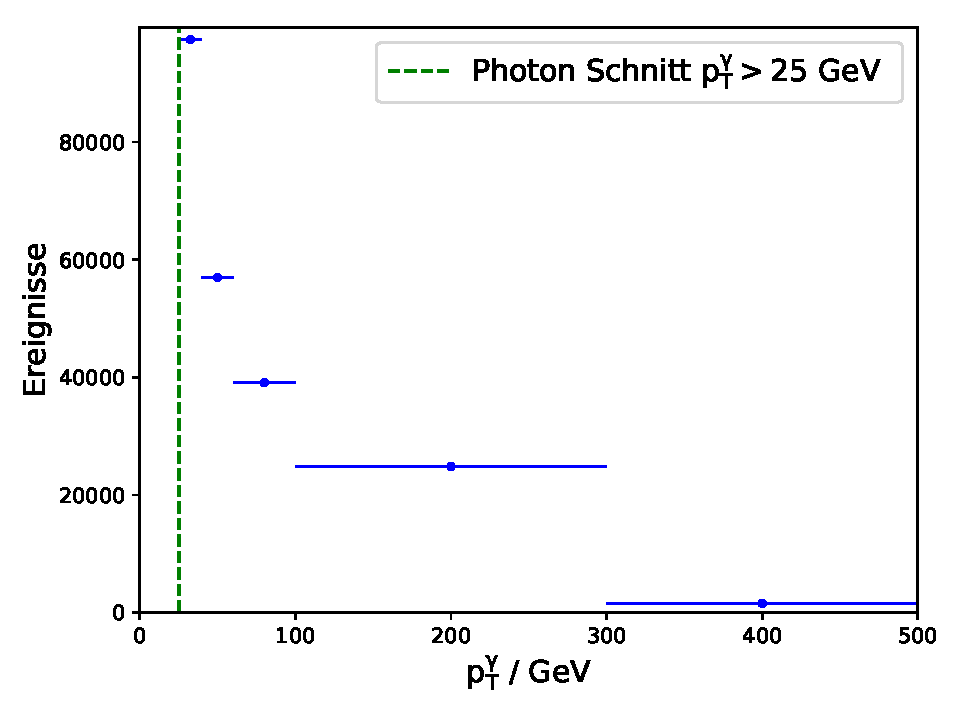
\includegraphics[width=\textwidth]{Plots/photon_pt_Cms.pdf}
      \subcaption{CMS}
    \end{subfigure}
    \begin{subfigure}[c]{0.5\textwidth}
      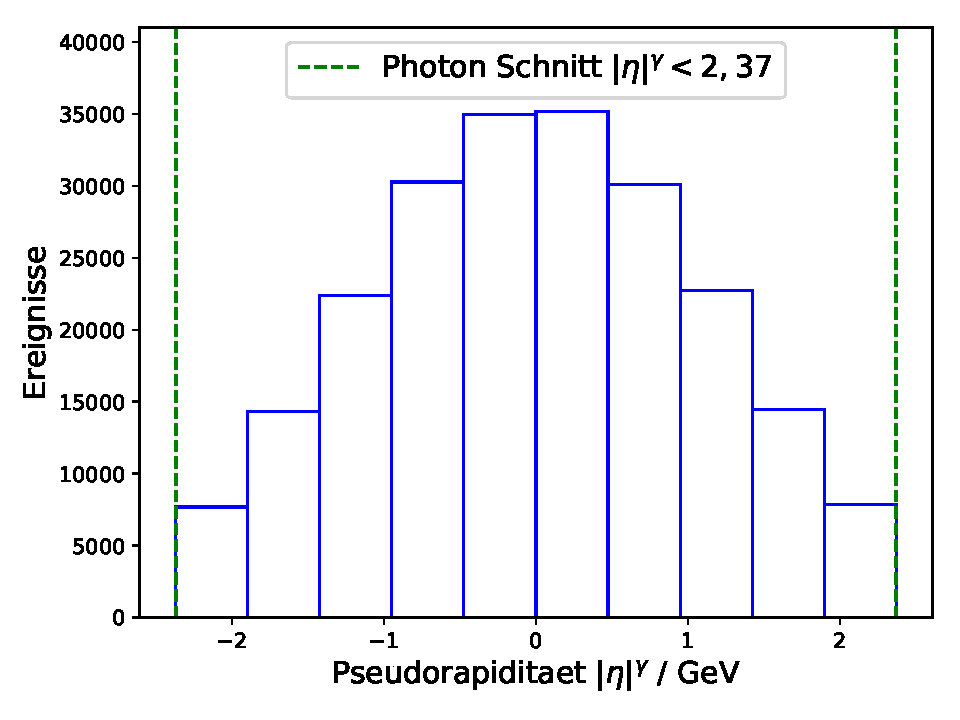
\includegraphics[width=\textwidth]{Plots/photon_eta_Atlas.pdf}
      \subcaption{ATLAS}
    \end{subfigure}
    \begin{subfigure}[c]{0.5\textwidth}
      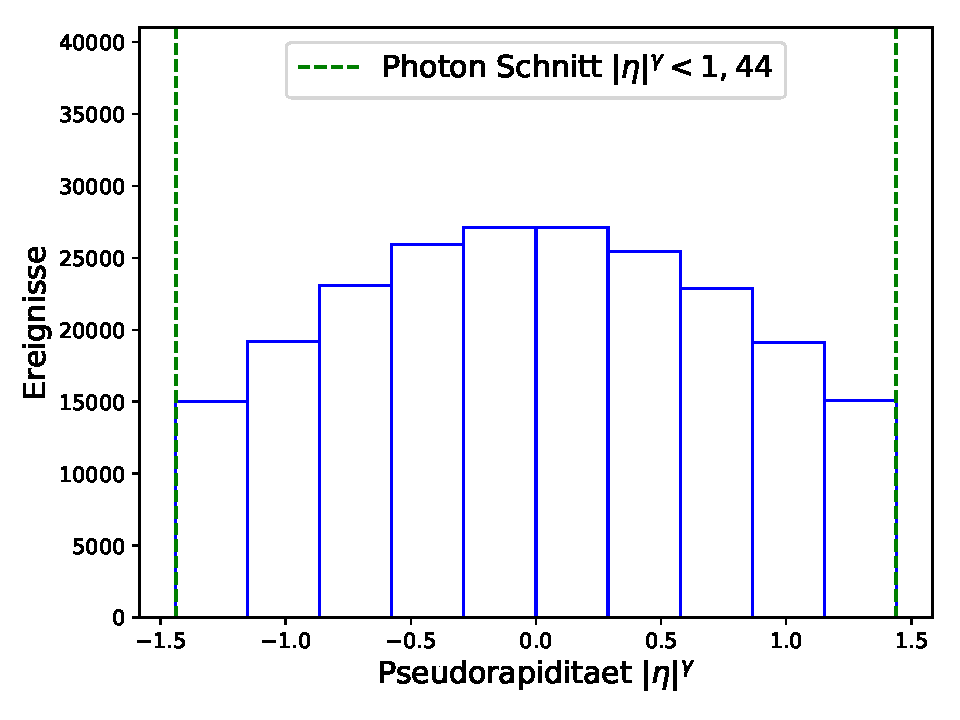
\includegraphics[width=\textwidth]{Plots/photon_eta_Cms.pdf}
      \subcaption{CMS}
    \end{subfigure}
    \caption{Verteilungen der Transversalimpulse und der Pseudorapidität der Photonen. Die grünen Linien representieren die von ATLAS und CMS verwendeten Schnitte. Die verwendeten Datensätze stammen aus Simmulationen mit MadGraph5.}
    \label{fig:schnitte}
\end{figure}
Um einen möglichst genauen Faktor zwischen den gemessenen Phasenräumen zu erhalten, wird eine Rechnung in der nächst-führenden Ordnung (\textit{next-to-leading-oder}, NLO) angestrebt. Dies ist bei MG für die expliziten Endzustände nicht möglich. Daher bietet es sich an, den Prozess $p~p~$\textrightarrow$~t~\bar{t}~\gamma$~ ohne diese, sowohl in LO als auch in NLO zu simulieren. Daraus kann im Anschluss ein $k$-Faktor als Näherung zwischen den beiden Ordnungen berechnet werden.\\
Damit ergeben sich folgende Wirkungsquerschnitte in der LO-Rechnung:
\begin{align}
  \sigma^{\text{ATLAS}}_{\text{LO}} &= 682,8 \pm 3,9~ \si{\femto\barn}\\
  \sigma^{\text{CMS}}_{\text{LO}} &= 361,6 \pm 1,5~ \si{\femto\barn}
\end{align}
und folgende Werte in der NLO-Rechnung:
\begin{align}
  \sigma^{\text{ATLAS}}_{\text{NLO}} &= 452,5 \pm 1,2~ \si{\femto\barn}\\
  \sigma^{\text{CMS}}_{\text{NLO}} &= 243,6 \pm 0,73~ \si{\femto\barn}.
\end{align}
Diese Wirkungsquerschnitte lassen sich durch Multiplizieren mit dem Verzweigungsverhältnis (\textit{branching ratio}, $\mathrm{BR}$) für den semileptonischen Zerfall in die, der expliziten Endzustände umrechnen. Das Verzweigungsverhältnis gibt die Wahrscheinlichkeit an, dass ein Zustand in einen bestimmten Endzustand zerfällt und liegt in diesem Fall bei $\mathrm{BR}=\SI{30}{\percent}$. Werden die Wirkungsquerschnitte nun mit der $\mathrm{BR}$ multipliziert und der NLO-Wert durch den der LO-Rechnung geteilt, ergibt sich folgender $k$-Faktor für ATLAS und CMS:
\begin{align}
  k_{\text{ATLAS}} &= \frac{0,3 \cdot 682,8~ \si{\femto\barn}}{0,3 \cdot 452,5~ \si{\femto\barn}} = 1,509\\
  k_{\text{CMS}} &= \frac{0,3 \cdot 361,6~ \si{\femto\barn}}{0,3 \cdot 243,6~ \si{\femto\barn}} = 1,484.
\end{align}
Auf Grund ihrer geringen Größe wurden die Fehler hier vernachlässigt. Unter Anwendung dieser $k$-Faktoren auf die zu Beginn bestimmten Produktionswirkungsquerschnitte ergibt sich der Phasenraumfaktor $f$ zwischen den gemessenen Phasenräumen von ATLAS und CMS zu:
\begin{align}
  f = \frac{1,509 \cdot 146,5~ \si{\femto\barn}}{1,484 \cdot 49,29~ \si{\femto\barn}} = 3,0221
\end{align}
Auch bei der Bestimmung mit einer Näherung für die NLO-Rechnung ergibt sich erneut ein Faktor der nahe an der drei liegt. Somit wird der CMS Phasenraum durch Multiplizieren mit einem Phasenraumfaktor von genau drei in den von ATLAS transformiert. Dabei ergeben sich die folgenden Produktionswirkungsquerschnitte:
\begin{align}
  \sigma^{fid(A), \text{CMS}}_{t\bar{t}\gamma, e} &= 410 \pm 140~ \si{\femto\barn}\\
  \sigma^{fid(A), \text{CMS}}_{t\bar{t}\gamma, \mu} &= 350 \pm 100~ \si{\femto\barn}.
\end{align}
Problematisch ist, dass bei dieser Rechnung über die Unsicherheit extrapoliert wird. Jedoch ist unklar, ob diese nicht nur im gemessenen CMS Phasenraum gültig sind. Diese Umrechnung wird trotzdem gewählt, da es sich lediglich um eine erste Näherung für die Vereinheitlichung der beiden Referenzphasenräume handelt. Dies bedarf weitergehender Studien durch eine aufwändigere Betrachtung der Unsicherheiten.
%
%
\chapter{Kombination der Messungen \texorpdfstring {$t\bar{t}\gamma$}{math}}
In diesem Kapitel wird die Vereinheitlichung der ATLAS und CMS Messungen unter der Verwendung des Ergebnisses aus dem Kapitel~\ref{phasencms} beschrieben. Hierbei ist zu beachten, dass die Kombination zuerst einmal unter der Annahme erfolgt, dass zwischen den drei Messergebnissen keine Korrelationen vorliegen. Um diese Annahme zu rechtfertigen, wird anschließend eine Korrelationsstudie für die Korrelation zwischen den beiden CMS Messungen durchgeführt.

\section{Gesamtkombination}
\label{kombi}
Wird eine unkorrelierte Kombination des angegebenen Produktionswirkungsquerschnitts von ATLAS und der in den gemessenen Phasenraum von ATLAS erweiterteten Messungen von CMS mit dem EFTfitter durchgeführt, ergibt sich der Wirkungsquerschnitt von $t\bar{t}\gamma$ zu:
\begin{align}
  \sigma_{\text{Kombi}} = 149,79 \pm 17,57~ \si{\femto\barn}.
\end{align}
Auffällig ist, dass das kombinierte Ergebnis sehr dicht an dem von ATLAS gemessenen Wert liegt.
Dies ist damit zu begründen, dass der EFTfitter eine Gewichtung der gegebenen Messungen anhand ihrer Unsicherheiten durchführt.
Durch die Extrapolation über die Unsicherheiten der CMS Messungen liegen diese in der selben Größenordnung wie die Nominalwerte, sodass diese Wirkungsquerschnitte bei der Berechnung der Kombination des EFTfitters nur sehr gering beitragen. Bei der Betrachtung der gaußförmigen Verteilungen um den gemessenen Produktionswirkungsquerschnitt in Abbildung~\ref{fig:gau} fällt auf, dass die Verteilungen für die CMS Messungen deutlich breiter sind und somit der Informationsgehalt für die ATLAS Messung höher ist. Dies erklärt die geringe Gewichtung der CMS Messungen durch den EFT-Fitter.\\
Dieses Ergebnis motiviert neben den Ergebnissen aus Kapitel~\ref{phasencms} ebenfalls eine genauere Betrachtung der Unsicherheiten und ihrer Gültigkeit in dem erweiterten Phasenraum. Zudem bietet es sich an, eine Korrelationsstudie durchzuführen, da für diese erste Kombination die Messungen als unkorreliert angenommen wurden.

\begin{figure}
  \centering
  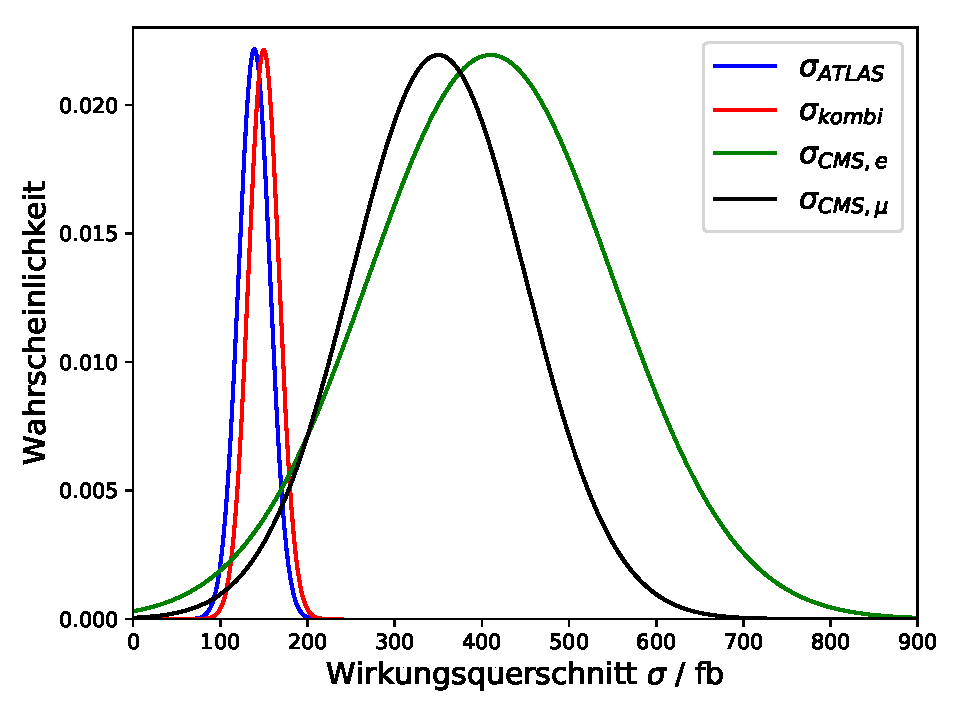
\includegraphics[width=0.8\textwidth]{Plots/gauss.pdf}
  \caption{Veranschaulichung der gaußverteilten Unsicherheiten um den Mittelwert der verschiedenen Messungen.}
  \label{fig:gau}
\end{figure}

\section{Korrelationsstudie}
Um eine unkorrelierte Kombination der drei Messungen zu rechtfertigen, wird eine Korrelationsstudie durchgeführt. Dabei wird zunächst nur eine Korrelation zwischen den beiden CMS Messungen untersucht. Hierfür werden die Ergebnisse aus Kapitel~\ref{phasencms} verwendet. Die verwendete Korrelationsmatrix ist symmetrisch, positiv semidefinit und hat die Form:
\begin{align}
  \text{Corr}_{\sigma,\text{CMS}}\,=\begin{pmatrix}
  1 & \rho_{e, \mu}\\
  \rho_{\mu, e} & 1
  \end{pmatrix}.
  \label{eqn:matrix1}
\end{align}
Aus diesem Grund wird für eine erste Betrachtung $\rho_{e, \mu}= \rho_{\mu, e}$ im Bereich $[-0,9~,~0,9]$ in $0,1$ Schritten variiert. Eine Kombination der beiden semileptonischen Produktionswirkungsquerschnitte von CMS unter Verwendung der Korrelationsmatrix $\text{Corr}_{\sigma,\text{CMS}}$ ist in Abbildung~\ref{fig:corrcms} dargestellt. Dabei lässt sich ein nahezu linearer Verlauf erkennen, der lediglich im Bereich hoher positiver Korrelationen abweicht. Da keine Effekte zu erkennen sind, scheint die Annahme, dass die Messungen nicht korreliert sind gerechtfertigt zu sein. Die großen Fehlerbalken lassen sich auf die großen Unsicherheiten der beiden Messungen zurückführen. Zudem wachsen sie bei einer positiven Korrelation weiter an, da die Messungen beide stärker gewichtet werden. Bei der negativen Korrelation wird hingegen die Gewichtung der zweiten Messung immer geringer, sodass bei einer großen, negativen Korrelationen eine Messung und damit ihre Unsicherheit sehr gering beiträgt.\\
Um ein möglichst genaues Ergebnis zu erhalten, wird nun noch einmal eine Korrelationsstudie zwischen den CMS-Messungen bei der Kombination mit der ATLAS Messung durchgeführt. Die entsprechende Korrelationsmatrix hat die Form:
\begin{align}
  \text{Corr}_{\sigma,\text{CMS}}\,=\begin{pmatrix}
  1 & 0 & 0\\
  0 & 1 &\rho_{e, \mu}\\
  0 & \rho_{\mu, e} & 1
  \end{pmatrix}.
  \label{eqn:matrix2}
\end{align}
In diesem Fall wird die Korrelation $\rho_{e, \mu}= \rho_{\mu, e}$ ebenfalls im Bereich $[-0,9~,~0,9]$ variiert, da die Matrix dort positiv semidefinit ist. Bei der Betrachtung von Abbildung~\ref{fig:corrca} fällt deutlich auf, dass der EFTfitter die beiden CMS-Messungen nicht stark gewichtet. Die Ursache dafür wird im Kapitel~\ref{kombi} genauer erläutert. Aus diesem Grund sind die Fehlerbalken deutlich kleiner als bei der Korrelationstudie, die ausschließlich zwischen den CMS Produktionswirkungsquerschnitten durchgeführt wurde. Eine Abweichung wird lediglich bei sehr großen negativen Korrelationen beobachtet.
Dies lässt sich damit erklären, dass der EFTfitter durch die Korrelation die CMS Messungen stärker gewichtet. Im restlichen Verlauf wird auf Grund der hohen Fehler dieser Messungen die ATLAS Messung stärker gewichtet, sodass sich auch die korrelierte Kombination stark dem ATLAS Messwert annähert.\\
\begin{figure}
  \centering
  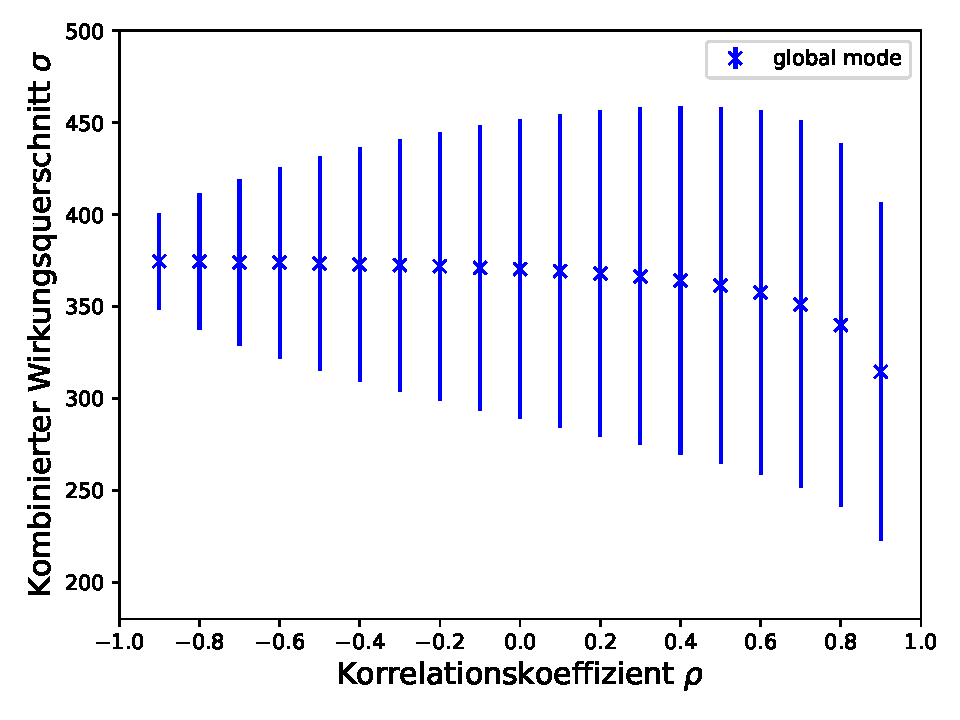
\includegraphics[width=0.7\textwidth]{Plots/corr_CMS.pdf}
  \caption{Untersuchung der Auswirkung verschiedener Korrelationen zwischen $[-0,9~,~0,9]$ zwischen den beiden semileptonischen Produktionswirkungsquerschnittmessungen von CMS.}
  \label{fig:corrcms}
\end{figure}
\begin{figure}
  \centering
  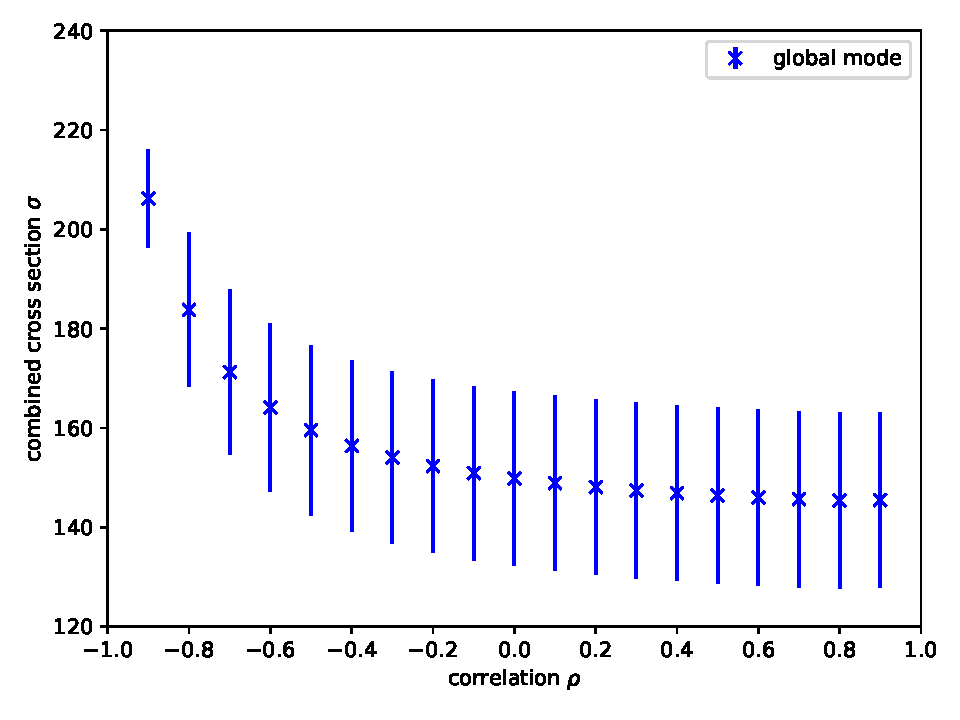
\includegraphics[width=0.7\textwidth]{Plots/fcorr_cms.pdf}
  \caption{Untersuchung der Auswirkung verschiedener Korrelationen zwischen $[-0,9~,~0,9]$ zwischen den beiden semileptonischen Produktionswirkungsquerschnittmessungen von CMS, bei einer Kombination mit der Messung von ATLAS.}
  \label{fig:corrca}
\end{figure}
\begin{figure}
  \centering
  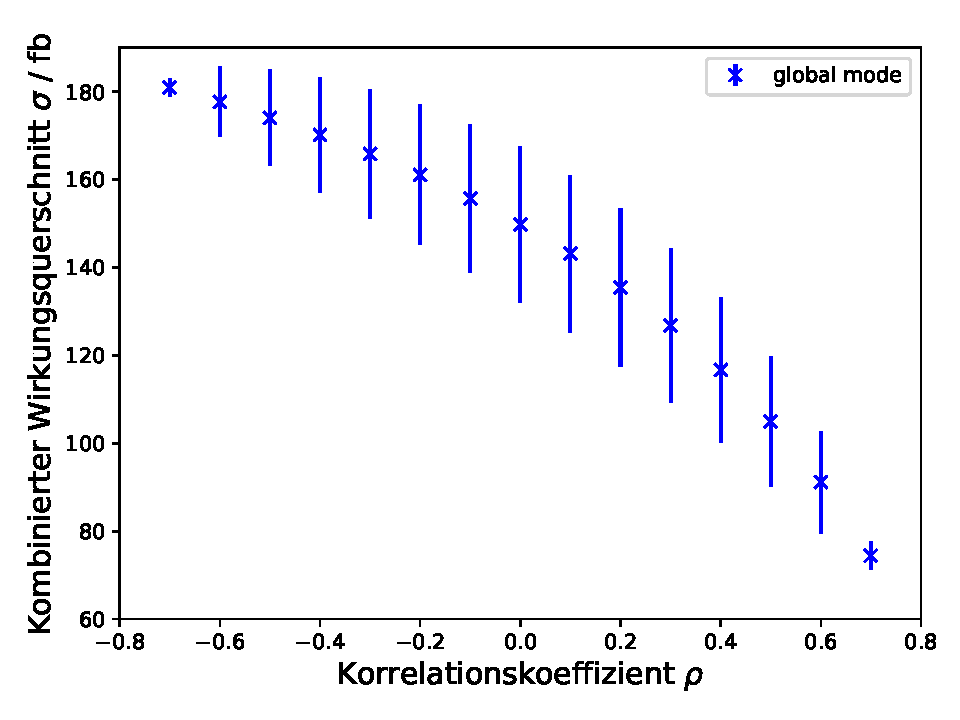
\includegraphics[width=0.7\textwidth]{Plots/corr_CA.pdf}
  \caption{Untersuchung der Auswirkung verschiedener Korrelationen zwischen $[-0,7~,~0,7]$ zwischen den beiden semileptonischen Produktionswirkungsquerschnittmessungen von CMS und der ATLAS Messung.}
  \label{fig:corrCA}
\end{figure}
Zuletzt wird die Korrelation zwischen der ATLAS Messung und den CMS Messungen untersucht. Die dazu verwendete Korrelationsmatrix hat die Form:
\begin{align}
  \text{Corr}_{\sigma,\text{CMS}}\,=\begin{pmatrix}
  1 & \rho_{e, \mu} & \rho_{e, \mu}\\
  \rho_{e, \mu} & 1 &0\\
  \rho_{e, \mu} & 0 & 1
  \end{pmatrix}
  \label{eqn:matrix2}
\end{align}
und die Korrelation wird entsprechend in $0,1$ Schritten im Bereich $[-0,7~,~0,7]$ variiert. In Abbildung~\ref{fig:corrCA} sind die sich ergebenden Ergebnisse dargestellt. Es fällt deutlich auf, dass sich kein Verlauf einstellt, der sich einem gewissen Bereich annähert. Dies deutet darauf hin, dass die Messungen des $t\bar{t}\gamma$ Produktionswirkungsquerschnitts korreliert sind.

\section{Interpretation der Ergebnisse der Kombination}
Zusammenfassend lässt sich feststellen, dass eine unkorrelierte Kombination der drei Messungen des Produktionswirkungsquerschnitts~$t\bar{t}\gamma$ nicht sinnvoll ist.
Dies liegt zum Einen an der Erweiterung des Phasenraums der CMS Messungen und der Extrapolation der Unsicherheiten. Es ist zu vermuten, dass diese im gemessenen Phasenraum von ATLAS nicht gültig sind. Mögliche Lösungen wären zum Einen genauere Rechnungen, um den Faktor $f$ zwischen den Phasenräumen nicht über eine Näherung zwischen LO- und NLO-Rechnungen bestimmen zu müssen. Zum Anderen wäre es möglich die ATLAS Messung des Produktionswirkungsquerschnitts in den CMS Phasenraum zu transformieren. In diesem Fall werden die Unsicherheiten durch die Extrapolation nicht vergrößert, sodass der EFTfitter alle drei Messungen stärker gewichtet.
Zum Anderen zeigen die Ergebnisse aus der Korrelationsstudie, dass die Annahme, dass die Messungen nicht korreliert sind, nur für die beiden CMS Messungen gerechtfertigt ist. Für die Korrelation zwischen der ATLAS und den CMS Messungen bedarf es jedoch noch weiterer Studien.
Da unter den in dieser Arbeit getätigten Annahmen die Kombination der Messungen nahe an dem ATLAS Wert liegt und verschiedene Faktoren dafür sprechen, dass die beiden Messungen hinsichtlich ihrer Unsicherheiten und Korrelationen erst weiter untersucht werden müssen, wird für die weitere Arbeit nur die ATLAS Messung verwendet.
%
%
\chapter{EFT-Modell mit MG5}
In diesem Kapitel erfolgt eine Variation der Wilson-Koeffizienten mit Hilfe eines EFT Modells für MG. Dies ermöglicht die Berechnung eines Modells der Wirkungsquerschnitte für den EFTfitter mit dessen Hilfe später die Wilson-Koeffizienten bestimmt werden können.

\section{Zusammensetzung des Wirkungsquerschnitts}
Der Fit des EFTfitters basiert auf einem funktionellen Zusammenhang zwischen den Observablen, in diesem Fall den Wirkungsquerschnitten, und den Operatoren höherer Ordnung. Diese Abhängigkeit wird durch das implementierte Modell und dem entsprechend mit der Likelihood ausgedrückt.\\
Für die Berechnung des Wirkungsquerschnitts werden alle zugehörigen Feynman-Graphen, sowohl die des SM, als auch die der EFT-Operatoren, betrachtet. Daher ergibt sich der Wirkungsquerschnitt zu:
\begin{align}
  \sigma = \sigma_{SM} + \frac{1}{\Lambda^2} \sum_{i} C_i \sigma_i^\text{interf.} + \frac{1}{\Lambda^4} \sum_{i \leq j} C_i C_j \sigma_{ij}^\text{BSM} + \mathcal{O} \left(\frac{1}{\Lambda^6}\right).
\end{align}
Die einzelnen Wirkungsquerschnitte $\sigma_i$ besitzen eine quadratische Abhängigkeit von den Wilson-Koeffizienten $C_i$ und die BSM-Beiträge in führender Ordnung ergeben sich durch die Interferenz zwischen dem SM und der BSM-Physik. Dies liegt unter Anderem daran, dass die Beiträge durch die Interferenz zwischen den BSM-Physik-Beiträgen untereinander mit $\frac{1}{\Lambda^4}$ unterdrückt sind. Um trotzdem ein möglichst genaues Modell für die Abhängigkeit der Wirkungsquerschnitte von den Wilson-Koeffizienten zu erhalten, müssen auch diese Beiträge betrachtet werden. Dies wurde bereits in dem Papier\cite{Wilson-Beiträge} untersucht. Zur Bestimmung des Modells ist es zudem notwendig die Wirkungsquerschnitte für verschiedene Konfigurationen der Wilson-Koeffizienten zu bestimmen.

\section{Variation der Wilson-Koeffizienten mit MadGraph5}
Eine Möglichkeit die Wilson-Koeffizienten zu variieren ist mit Hilfe eines MG Modells, dass Operatoren der Massendimension sechs enthält und damit eine Berechnung der Wirkungsquerschnitte unter dem Einfluss dieser ermöglicht. Dazu wird in MadGraph5 das TEFT\_EF UFO Modell\cite{EFTModell} eingebunden. Dies erlaubt NLO Rechnung in der QCD und enthält alle für die Top-Quark-Physik relevanten Operatoren der Dimension sechs.\\
Die Berechnung erfolgt mit dem genannten Modell in NLO in QCD unter der Verwendung des $\text{CTEQ}6\text{L}1$ PDF Sets. Zudem wird die Energieskala auf $\SI{1}{\tera\electronvolt}$ festgelegt. Unter diesen Vorraussetzungen wird der Prozess $pp~\rightarrow~t\bar{t}~\gamma$ mit den von ATLAS genutzten Schnitten implementiert.\\
Da die Berechnung statistische Unsicherheiten enthält, bietet es sich an anstatt nur genügend viele Berechnungen der Monte Carlo Wirkungsquerschnitte $\sigma_{MC}$ für ein bestimmtes Gleichungssystem zur Bestimmung der Wirkungsquerschnitte $\sigma_i$ durchzuführen sondern mehr. Zudem werden genauere Ergebnisse erhalten, wenn sowohl Berechnungen bei denen nur ein Wilson-Koeffizient angeschaltet ist, als auch welche beidenen mehrere oder sogar alle betrachtet werden, getätigt werden.\\
Die berechneten Monte Carlo Wirkungsquerschnitte:
\begin{align}
  \sigma_{MC}({C_i}) = \sigma_{SM} + \sum_{i} C_i \frac{\sigma_i}{\Lambda^2} + \sum_{i \leq j} C_i C_j \frac{\sigma_{ij}}{\Lambda^4} + \mathcal{O}(\frac{1}{\Lambda^6})
\end{align}
bilden die Stützstellen zur späteren Bestimmung der gesuchten Wirkungsquerschnitte. Mit Hilfe des Vakuumerwartungswert des Higgs $\SI{246}{\giga\electronvolt}$ und der Wahl $\Lambda = \SI{1}{\tera\electronvolt}$ lassen sich die $\sigma_{MC}$ in natürliche Einheiten umrechnen. Unter Vernachlässigung de Terme der Ordnung $\mathcal{O}(\frac{1}{\Lambda^6})$ ergeben sie sich zu:
\begin{align}
  \sigma_{MC}({\tilde{C_i}}) \approx \bar{\sigma}_{SM} + \sum_{i} \tilde{C_i} \bar{\sigma_i} + \sum_{i \leq j} \tilde{C_i} \tilde{C_j} \bar{\sigma}_{ij}.
\end{align}
Hierbei sind die $\tilde{C}_i = \frac{v^2}{\Lambda^2} C_i$.
Bei der Berechnung des $t\bar{t}\gamma$ Produktionswirkungsquerschnitts können, wie in Kapitel~\ref{top} bereits erwähnt, die Operatoren $O_{tG}$, $O_{tW}$ und $O_{tB}$ beitragen. Damit ergibt sich die Interpolationsfunktion zu:
\begin{align}
  \sigma_{t\bar{t}\gamma, MC}({\tilde{C}_{tG}, \tilde{C}_{tW}, \tilde{C}_{tB}}) = \bar{\sigma}_{SM} + \tilde{C}_{tG}\bar{\sigma}_{tG} + \tilde{C}_{tW}\bar{\sigma}_{tW} + \tilde{C}_{tB}\bar{\sigma}_{tB}\\
  + \tilde{C}_{tG}^2\bar{\sigma}_{tGtG} + \tilde{C}_{tW}^2\bar{\sigma}_{tWtW} + \tilde{C}_{tB}^2\bar{\sigma}_{tBtB}\\
  + \tilde{C}_{tG} \tilde{C}_{tW}\bar{\sigma}_{tGtW} + \tilde{C}_{tG} \tilde{C}_{tB}\bar{\sigma}_{tGtB} + \tilde{C}_{tW} \tilde{C}_{tB}\bar{\sigma}_{tWtB}
\end{align}
und es müssen insgesamt zehn Parameter $\bar{\sigma_i}$ und $\bar{\sigma}_{ij}$ bestimmt werden. Dazu werden die Wilson-Koeffizienten $C_{tG}$, $C_{tW}$ und $C_tB$ im Bereich $[-30~,~30]$ variiert. Um erneut nur die semileptonischen Endzustände zu betrachten, müssen auch in diesem Fall die $\sigma_{t\bar{t}\gamma, MC}$ mit dem $\mathrm{BR} = \SI{30}{\percent}$ multipliziert werden. Aus diesen Berechnungen lassen sich dann mit der Methode der kleinsten Quadrate die gesuchten Parameter bestimmen, aus denen sich schließlich das Modell für den EFTfitter ergibt.

\section{Plots mit Schnitten}
Die Schnitte mit der sich ergebenen Hyperebene sind parabelförmig, wenn nur ein Wilson-Koeffizient variiert wird. Dies ist zu erwarten, da die Zusammensetzung der Monte Carlo Wirkungsquerschnitt auch aus quadratischen Anteilen besteht. Die direkt an der Photonabstrahlung beteiligten Wilson-Koeffizienten $C_{tW}$ und $C_{tB}$ folgen ziemlich genau diesem parabelförmigen Verlauf. Dies ist in Abbildung~\ref{fig:WtW} und~\ref{fig:WtB} veranschaulicht. Lediglich die berechneten Wirkungsquerschnitte für den Wilson-Koeffizienten $C_{tG}$ weisen stärke Abweichungen auf, dies ist in Abbildung~\ref{fig:WtG} dargestellt.\\
Die Ursache hierfür könnte bei (...)liegen.
\begin{figure}
  \begin{subfigure}[c]{0.5\textwidth}
    \centering
    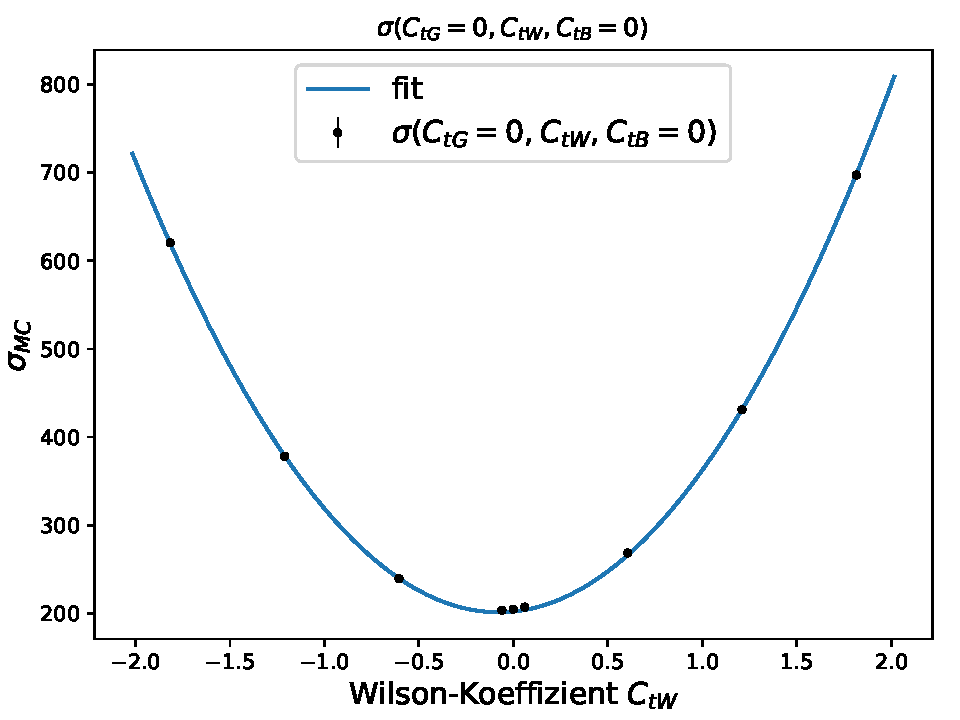
\includegraphics[width=\textwidth]{Plots/combi_plot_tW.pdf}
    \subcaption{Verlauf für $C_tW$ mit $C_{tB}=C_{tG}=0$.}
    \label{fig:WtW}
  \end{subfigure}
  \begin{subfigure}[c]{0.5\textwidth}
    \centering
    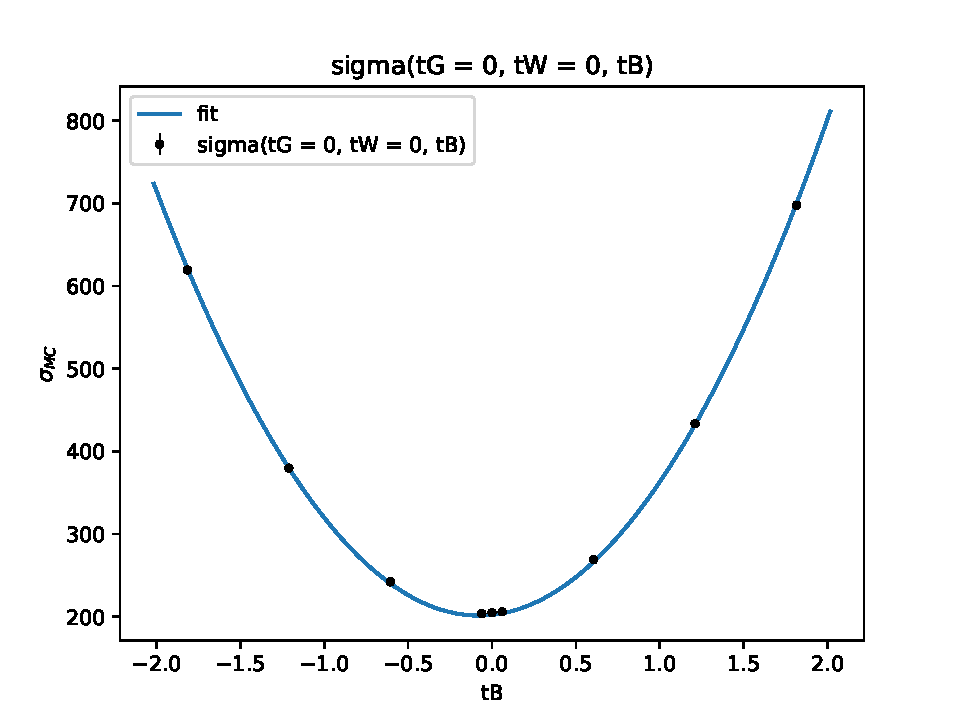
\includegraphics[width=\textwidth]{Plots/combi_plot_tB.pdf}
    \subcaption{Verlauf für $C_tB$ mit $C_{tW}=C_{tG}=0$.}
    \label{fig:WtB}
  \end{subfigure}
  \caption{Graphische Darstellung des parabelförmigen Verlaufs der Wirkungsquerschnitte für die Betrachtung einzelner Wilson-Koeffizienten.}
\end{figure}
\begin{figure}
  \centering
  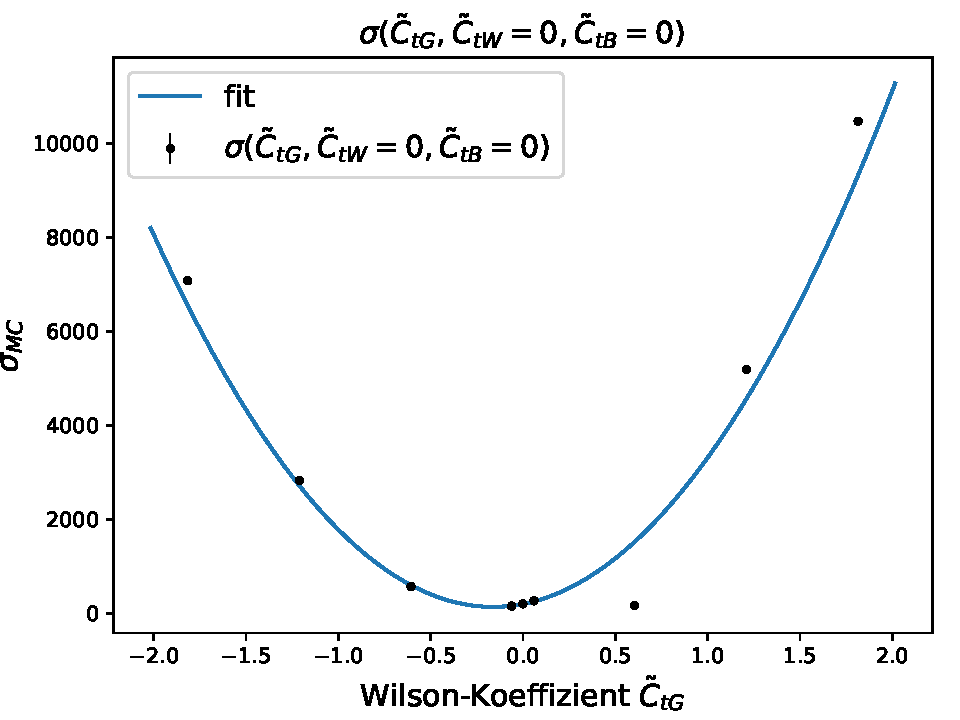
\includegraphics[width=0.5\textwidth]{Plots/combi_plot_tG.pdf}
  \caption{Graphische Darstellung des parabelförmigen Verlaufs der Wirkungsquerschnitte für den Wilson-Koeffizienten $C_{tG}$, wenn $C_{tW}=C_{tB}=0$ ist.}
  \label{fig:WtG}
\end{figure}

\section{MadGraph Modell für den EFTfitters}
\begin{align*}
  s_{SM}   &= 202.193110217 \pm 0.0293749106165\\
  s_tW   &= 21.6894366072 \pm 0.279039825848\\
  s_tB   &= 761.416032917 \pm 8.2990258513\\
  s_tG   &= 21.6811677276 \pm 0.337443892498\\
  s_tWtW &= 11.7700260688 \pm 0.000323156142251\\
  s_tBtB &= 48.4373822429 \pm 0.00172124829635\\
  s_tGtG &= 11.794900333 \pm 0.000390544938718\\
  s_tBtW &= 279.22019759 \pm 1.61033246225\\
  s_tWtG &= 6863.75881087 \pm -1.44115188502e+17\\
  s_tBtG &= -6483.30787401 \pm -1.4411518765e+17
\end{align*}
\textit{Die Frage ist hier halt ob diese angegebenen Fehler überhaupt aussagekräftig sind. Das ist ja eine statistische Abschätzung, die auch gewissen Annahmen beinhaltet.Bei einem so hochdimensionalem Fit ist das natürlich auch sehr anfällig bei Abweichungen.. und die sind besonders im Fall von $C_tG$ ja offensichtlich noch vorhanden.}
%
%
\chapter{EFT-Interpretation des \texorpdfstring {$t\bar{t}\gamma$}{math} Produktionswirkungsquerschnitts mit dem EFTfitter}

\section{Ergebnis für die Wilson-Koeffizienten}

\begin{figure}
    \centering
    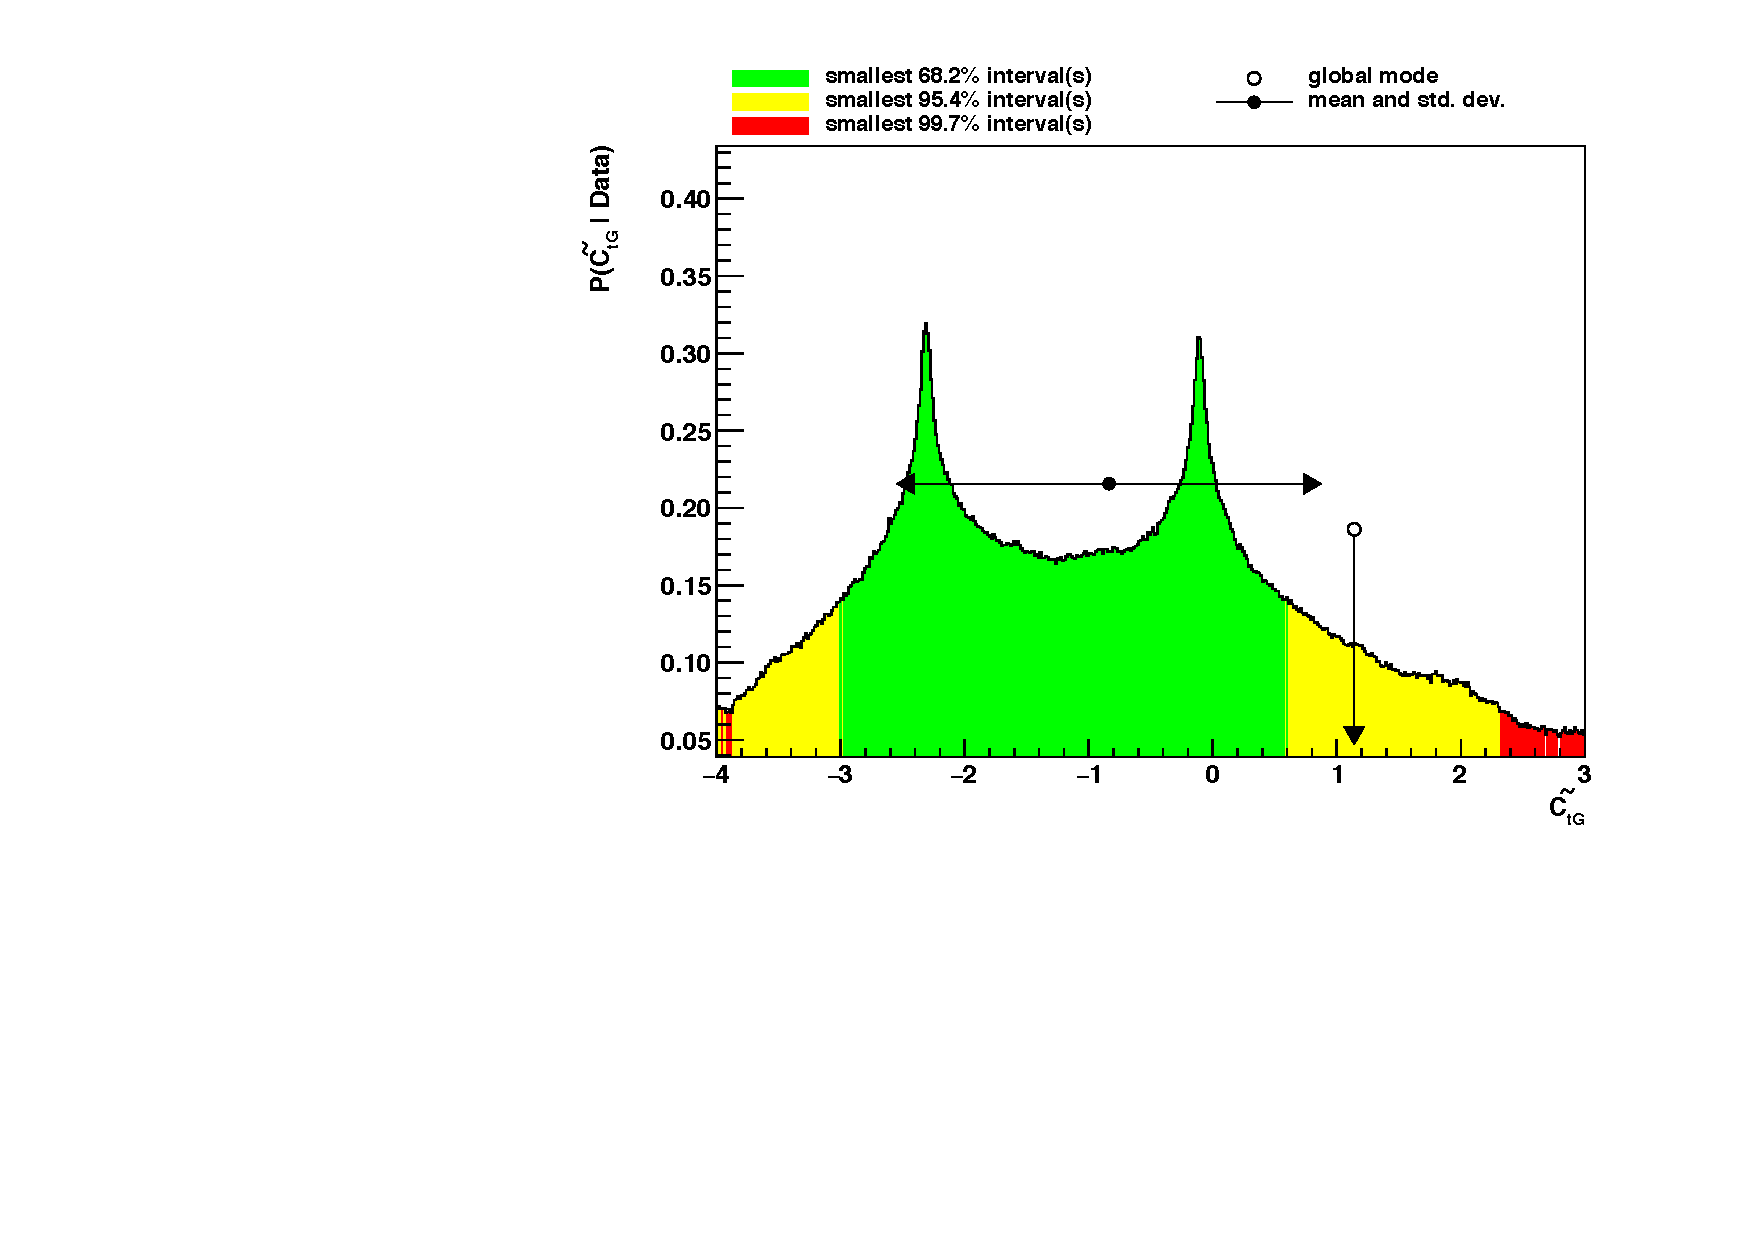
\includegraphics[width=0.8\textwidth]{Plots/result_CtG.pdf}
\end{figure}
\begin{figure}
    \centering
    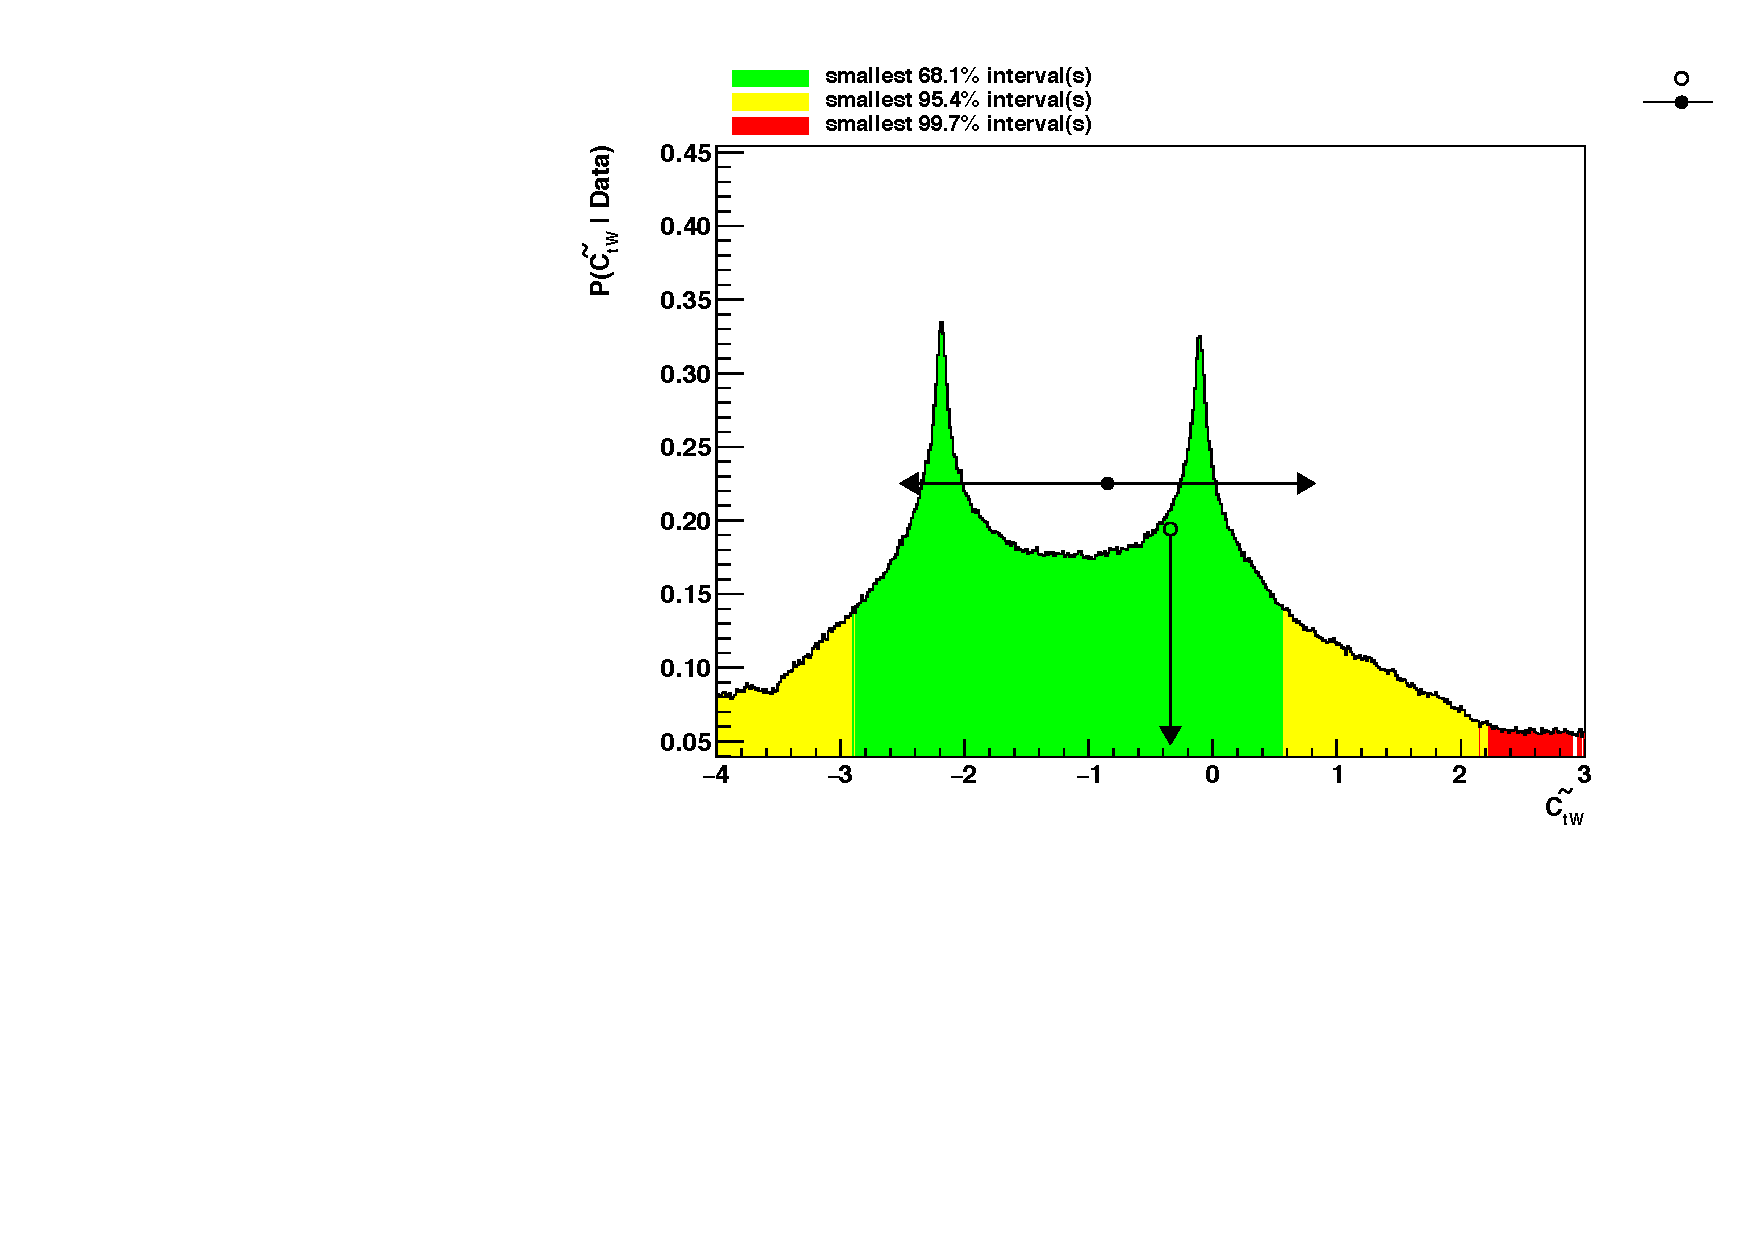
\includegraphics[width=0.8\textwidth]{Plots/result_CtW.pdf}
\end{figure}
\begin{figure}
    \centering
    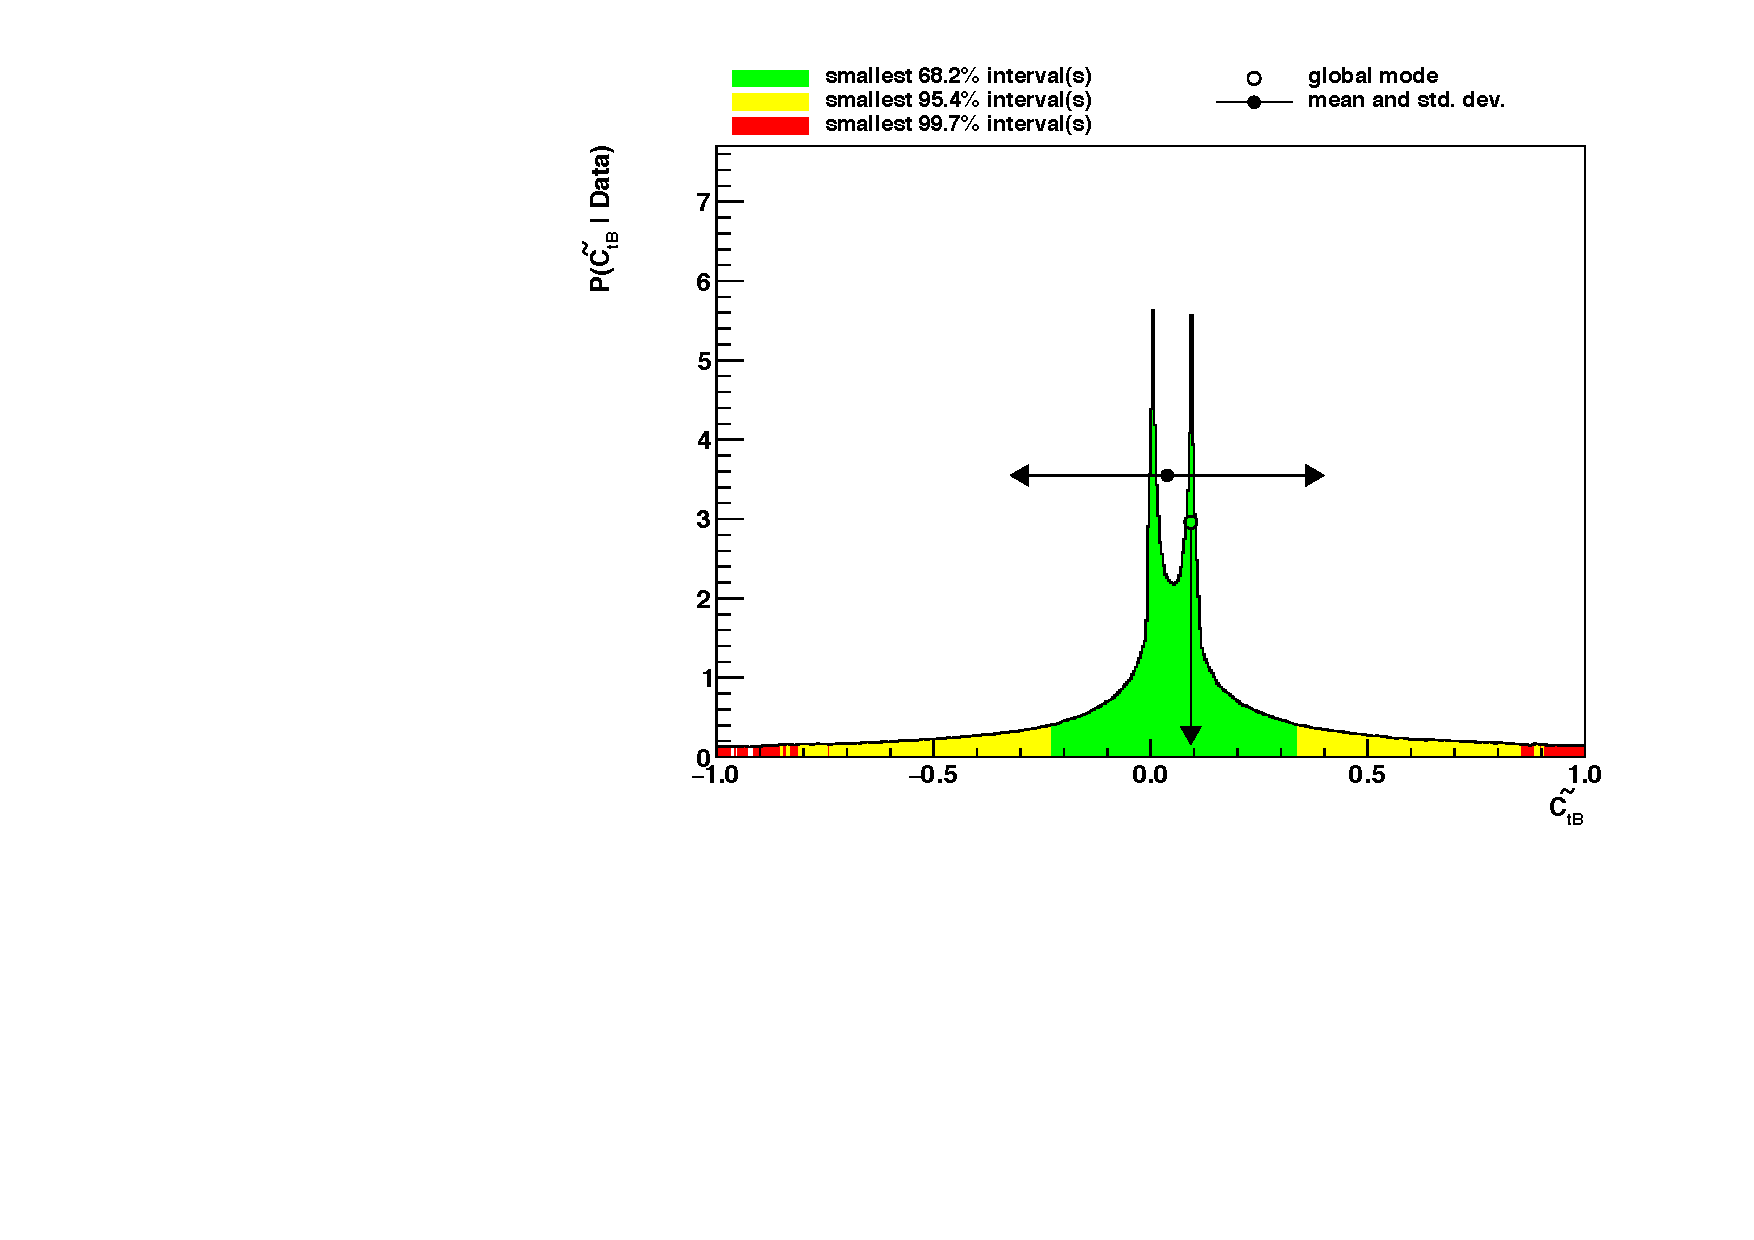
\includegraphics[width=0.8\textwidth]{Plots/result_CtB.pdf}
\end{figure}
